\documentclass[letterpaper, 10 pt, conference]{ieeeconf}

\overrideIEEEmargins

\usepackage{graphicx}
\usepackage{float}

\title{\LARGE \bf
Face-to-Face Authentication
}

\author{Matthew Suozzo}

\begin{document}

\maketitle
\thispagestyle{empty}
\pagestyle{empty}

%%%%%%%%%%%%%%%%%%%%%%%%%%%%%%%%%%%%%%%%%%%%%%%%%%%%%%%%%%%%%%%%%%%%%%%%%%%%%%%%
\begin{abstract}

Authentication is a persistent concern for end-users and corporations alike.
The increasing reliance of critical infrastructure on computing systems and their increasing complexity necessitate a more robust access control regime.
Multi-factor authentication solutions begin to address threats such as phishing but are ineffective against insider adversaries and already-compromised accounts.
To better address these threat models, multi-\emph{party} authentication systems are required.
We introduce Face-to-Face Authentication, a multi-party authentication system which is particularly resilient in insecure physical and network environments.

\end{abstract}

\section{Background}

  \textbf{Authentication}: The process of verifying that the user's claimed identity matches their actual identity or, more colloquially, `they are who they say they are.'

  \textbf{Authorization}: The process of verifying that the user's claimed identity is permitted to take the attempted action or `they're allowed to do what they're trying to do.'

  While these two concepts may appear somewhat disjoint, authorization is entirely reliant on being able to properly identify the user i.e. authentication.
  Making access control decisions is impossible if the system cannot reliably identify who is attempting the access.
  Or concretely, a policy that permits user A to take some action is not meaningful if there is no way to verify that a user is indeed user A.
  At the extreme, a policy might specify that a system only recognizes, and is only accessible to, a single user.
  In this case, authorization is completely subsumed by authentication: The assignment of identity is the only access-relevant decision.
  While access policies are rarely this trivial, they are often relatively simple so that the real complexity lies in authentication confidence.

  Authentication can take many forms but there is a common taxonomy used to group authentication methods:
  \begin{itemize}
      \item Something you know (e.g. a password)
      \item Something you have (e.g. a hardware token)
      \item Something you are (e.g. a fingerprint)
  \end{itemize}
  
  Recently, though, a new group of authentication methods, or ``factors," has emerged which defy classification in the existing taxonomy.
  They are broadly known as ``environmental" authentication factors which take into account ambient activity or measurements to influence an authentication decision.
  One example is an authentication system that correlates audio from the user's phone with that of their computer to establish proximity \cite{ambient}.
  This trend has been facilitated by smartphones as they can provide a platform on which hyper-localized sensing and/or computing may take place.
  Due to this proliferation of localized computation, metrics such as location, sound, RF, etc. are now possible to incorporate into these decisions.

  Individually, each class of authentication factors is often weak to a particular set of threat models.
  For instance, an attacker on the network can readily compromise the users' password by sniffing packets while a physical attacker can lift their fingerprints off of a used drinking glass.
  One way to address these individual shortcomings is to require the user to provide more than one factor.
  This defence-in-depth strategy is known as two-factor authentication (2FA) for just two methods or, in the more general case, multi-factor authentication (MFA).
  Given its expected greater security, MFA provides more confidence that the authentication can be trusted and, thus, that derivative authorization decisions are valid.

  A variant of MFA is multi-party authentication/authorization (MPA) whereby another user is required to take an action to complete the authorization flow.
  This action could be as simple as being present during the process or could require active involvement such as providing a credential.
  The other party may be restricted to peers (i.e. an equal in the organization/system), a supervisor, or may be any valid user in the system.
  MPA is often used to gate the most sensitive operations as it can limit the impact of a single bad actor with full access to the system.
  More precisely, MPA offers greater assurance in threat models where users inadvertently or maliciously misuse their authorization, known as ``insider threats."
  Another related (and far more common \cite{insider}) threat is that of a compromised user account as the user will, in their actions, appear to be malicious.

  The U.S. military has put MPA into wide use, primarily in service of physically and operationally securing nuclear weapons systems.
  The implementations are referred to by a number of different names but the underlying principle is known as the ``two-person rule."
  One example is the Air Force's requirement that Inter-continental Ballistic Missile silos be ``No-Lone Zones," areas where no fewer than two qualified personnel may be inside at any one time.
  Similarly, the Navy requires the presence and credentials of two qualified individuals in order to grant access to sensitive cryptographic material \cite{navy}.
  Not only are insider risks salient in these situations, the consequences of unintentional mistakes would be too grave to permit unilateral access to any individual.

  Outside of military applications, there are a number of other domains that utilize MPA:
  PCI (payment processing), HIPAA (medicine), and SOX (finance) compliance regimes consider manual review (i.e. two-person auth) for all code, configuration, etc. changes as either a mandate or a best practice \cite{pci} \cite{mscomp}.
  Another more modern use of MPA is in Facebook's ``Trusted Contacts" account recovery scheme where other Facebook accounts are authorized to help you in the event you get locked out of your account \cite{fb}.

\section{Design} \label{design}

  \begin{figure*}
    \centering
    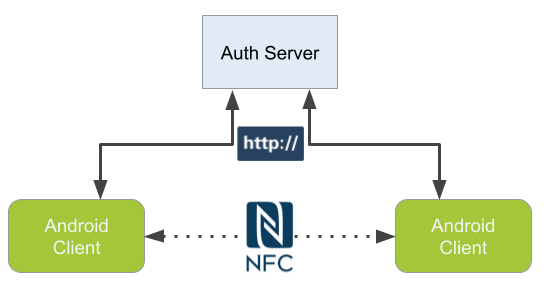
\includegraphics[width=300px]{component-diagram.png}
    \caption{A (very) high-level component diagram of the Face-to-Face Auth system.}
    \label{arch}
  \end{figure*}

  Face-to-Face (F2F) Auth is a multi-party, environmental authentication and/or authorization system designed to protect highly sensitive operations.
  A high-level diagram of the system components can be found in Figure \ref{arch}.
  It utilizes the communications capabilities of smartphones to tie environmental conditions, namely the physical presence of another party, to the authentication decision.
  In addition, the physically present party also needs to make an explicit approval of the authentication request.
  Together, these characteristics make this instantiation of multi-party authentication well-positioned to act as an authentication factor for high-assurance systems.
  A more in-depth analysis of the security properties of the system can be found in Section \ref{secproperties}.

  \subsection{Peer Authentication} \label{peerauth}

  From the authenticating user's perspective, the process works as follows:
  \begin{enumerate}
    \item A user (the ``primary") is prompted to get a credential by the authentication server upon attempting an operation
    \item The primary finds another user (the ``peer") and asks them to assist in the authentication
    \item The primary uses the client app to make the request to the peer by tapping their phones together
    \item The peer is prompted by their client app to decide whether they want to authenticate the primary
    \item Provided they accept, the peer taps their phone to the primary's
    \item And, finally, the primary reconnects to the authentication server with evidence of this exchange
  \end{enumerate}

  Prior to a device participating in primary or peer authentication, it must be registered with the authentication server.
  At a high level, this entails the device creating a keypair and sending the public key to the auth server at which point the server issues a client certificate and sends it to device.
  In a corporate environment, this exchange could be performed as part of the device provisioning workflow.
  Further detail on the device registration/provisioning process is provided in Section \ref{provisioning}.

  The ``tapping" referred to in the auth procedure uses Near-Field Communication (NFC), a short-range RF technology present in most modern Android devices, to transmit the data requisite to the protocol.
  NFC provides a number of desirable security properties such as a tight constraint on the distance it is able to transmit and, in this implementation, a refusal to receive messages when the device is locked.
  The communication between the client apps and the authentication server is done over mTLS (mutually-authenticated TLS) with the apps presenting the client certificate issued by the auth server.

  The authentication flow uses the following protocol to construct cryptographic evidence of the exchange:
  % U_y -> U_p {t_1, id_y, S_y{t_1, id_y}}
  % U_p -> U_y -> AS {t_1, id_y, S_y{t_1, id_y}, t_2, id_p, S_p{t_1, id_y, S_y{...}, t_2, id_p}}
  % AS -> U_y {<opaque access token>}
  
  $$ \{t_1, id_y, S_y(\leftarrow)\}\eqno{(U_y \rightarrow U_p)} $$
  $$ \{t_1, id_y, S_y\{\leftarrow\}, t_2, id_p, S_p\{\leftarrow\}\}\eqno{(U_p \rightarrow U_y \rightarrow AS)} $$
  $$ \{opaque\_access\_token\}\eqno{(AS \rightarrow U_y)} $$

  Where $U_y$ is the primary user, $U_p$ is the peer, $AS$ is the auth server, $t_1$ is the time at protocol start, $t_2$ is the time at auth response, $id_x$ is the name of user $x$, and $S_x\{\leftarrow\}$ is the signature of all elements to the left of the occurrence under the key owned by user $x$.

  The auth server performs a number of checks on the input before returning the access token, notably that the signatures verify using the associated public keys and that the timestamps provided are within a given period of time (e.g. 30 seconds of each other) and are not older than a given increment (e.g. a minute old).
  If these checks pass and the flow is completed, $U_y$ can provide the opaque access token on subsequent requests to the $AS$ (or through a proxy server) to access the gated operations.

  \subsection{Provisioning} \label{provisioning}
  The provisioning process registers a device with the auth server for future use in primary and peer authentication roles.
  % U_a -> AS {}
  % AS -> U_a {id_n}
  % U_a -> U_n {Url_AS, id_n}
  % U_n -> U_a -> AS {id_n, P_n}
  % AS -> U_a -> U_n {id_n, C_n}
  $$ \{\} \eqno{(U_a \rightarrow AS)} $$
  $$ \{id_n\} \eqno{(AS \rightarrow U_a)} $$
  $$ \{Url_{AS}, id_n\} \eqno{(U_a \rightarrow U_n)} $$
  $$ \{id_n, P_n\} \eqno{(U_n \rightarrow U_a \rightarrow AS)} $$
  $$ \{id_n, C_n\} \eqno{(AS \rightarrow U_a \rightarrow U_n)} $$

  Where $U_a$ is an admin-authorized user, $U_n$ is the new user, $Url_{AS}$ is the URL of the authentication server, $P_n$ is the public key generated by the new user, and $C_n$ is the client cert issued by the AS.

  The new user generates a signing key pair during provisioning with the secret key never leaving the device and the public key shared and stored by the auth server.
  The on-device generation of the private key is desirable because it means the signing key used by the client is never handled or read by any other principal in the system and so cannot be used to subvert the multi-party requirement.
  See the associated discussion in Section \ref{secproperties}.

  \subsection{Realms} \label{realms}
  Whenever a user ID is transmitted in the above protocol descriptions, it is actually accompanied by a scoping identifier called the ``security realm".
  This mechanism provides a 1:1 mapping of a user onto a group representing a set of mutual peers.
  This grouping can be used to mirror an organization (e.g. by domain ``mycorp.com") or subdivide one into even smaller silos (e.g. by team ``Security") to limit the set of valid peers for an authentication action.
  This feature can be extended in a number of ways which are touched on briefly in Section \ref{future}.

\subsection{Prototype Status} \label{prototype}
  The prototype implementation consists of a Golang server and Kotlin Android app client.
  The system performs the above authentication flow as well as the full provisioning flow, albeit with a minimal UI and a few missing features.

  The most significant work-in-progress feature is that of client certificate support.
  While the server supports them, the semantics of issuance and client handling are not yet fully implemented.
  The intention would be to store the client cert fingerprint in the server's device database.
  With each connection, an initial check would mandate a client cert be presented and would match that identity to a device.
  Again, the stubs for this logic are present in the server code.
  As for provisioning, the client cert would simply be issued by the server and sent down in the final server-to-new-client exchange, the content of which is currently ignored.
  The client cert would be stored by the client in the device profile and used to construct the \texttt{SSLConfig} for all future connections to the auth server.
  All this said, we include the references to client certs throughout as they are a key part of the design, regardless of the implementation status of the prototype.

  The prototype does not distinguish between admin and non-admin devices primarily due to the lack of robust client identification support (i.e. no client certificates).
  Once clients can be identified, this could be addressed with a manual whitelist provided to the server at startup or by some dynamic grouping mechanism.

  Another shortcoming of the prototype is UI support for multiple device profiles.
  While this is supported by the data model, there is no way to select the active device account from the client app.
  In the common case, though, a device will only be in a single organization and will likely only have one associated profile so this is a less relevant omission.

\section{Analysis} \label{security}

\subsection{Security Properties} \label{secproperties}
  There are a number of security advantages of the F2F Auth system.
  From provisioning to authentication, there is very little reliance on either physical or network security.
  NFC operates over very short ranges ($\sim$1-10cm) so eavesdropping or interference requires either very close proximity or a \emph{very} large antenna (\textgreater1m) \cite{surrey}.
  The auth prompt also requires both an unlocked device and an active touch by the user which would be extremely difficult to induce without the user's knowledge.
  Assuming the device requires strong authentication (either password or biometric), theft of a single device becomes much less of a risk to the overall system integrity.
  Combining this with NFC's low risk of unintentional peer authentication, the system can operate quite well in an uncontrolled, potentially hostile physical environment.

  Network risk is also mitigated by a number of factors.
  The auth server never processes a request without a mutual TLS connection (i.e. without the client presenting a certificate issued by the server).
  And since peer authentication is negotiated over NFC, it is largely immune to network-based attacks.
    
  The overall simplicity of the system is also a security benefit.
  Insecurity as a consequence of misuse is a common ailment of security systems where too much complexity is exposed to users.
  With F2F Auth, the user only needs to find another user and exchange phone taps to properly authenticate.
  No additional configuration or options are required, let alone provided, which leaves very few ways to misconfigure or misuse the app.

  Another benefit of F2F Auth is that the credential returned by the auth server is not a bearer token, it is only valid when connecting with the associated client certificate.
  Because the credential is bound to a device identity, it cannot be used to authenticate without that device's client certificate.
  Consequently, this weakens the confidentiality and integrity requirements for the token's storage and handling.

  As a result of being a multi-party authentication system, a single compromised device cannot forge or meaningfully influence the system to acquire an access token.
  During the authentication flow, the peer is sent metadata about the primary but instead of trusting this information on fiat, it contacts the auth server to retrieve the information instead.
  This mutual distrust between the principals removes the possibility that a compromised device could deceive a peer into authorizing a different user.

  \begin{figure*}
    \centering
    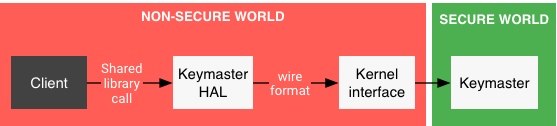
\includegraphics[width=350px]{access-to-keymaster.png}
    \caption{The structure of Android key management. The Keymaster API allows the private key to be generated on, and remain relegated to, a tamper-resistant hardware security module.}
    \label{keymaster}
  \end{figure*}

  One potential concern might be that an attacker with physical access to a device might be able to extract its identity and then use it to peer for another device.
  However Android's Keymaster management interface makes it impossible to extract (through software) the private key material \cite{androidkeys}.
  All signing operations are required to be performed outside of the kernel entirely in a secure coprocessor as shown in Figure \ref{keymaster}.
  In addition to the software inaccessibility of the key material, a new addition to the Android OS supports key storage in a hardware security module which provides physical tamper protection \cite{androidstrongbox}.

\subsection{Threat Model} \label{secattacks}
  Like any security system, F2F Auth is not perfect and must be evaluated based on its potential weaknesses.
  The design ideal is to make feasible attacks difficult, low-impact, and/or defended by other systems.

  \emph{Malicious/Coerced User:} If a user is blackmailed or maliciously motivated to attempt authentication, there is not much that can be done.
  The only impediment in the way of the attacker's success is the peer's approval.
  If the request is sufficiently out-of-character or unjustified, it's possible that the peer becomes suspicious and raises an alarm.
  That said, this is one of the most difficult threat models to combat because of the attacker is knowledgeable, motivated, and has the proper authority so most technical controls are moot.
  The best defence against this sort of attacker is to not have them be authorized at all: Limiting the set of users able to take an action reduces the risk of coercion and the capability of a potential insider.

  \emph{Compromised Non-admin Device:} If an attacker gets logical control of a device (say, code execution instead of physical access), they can compromise the client app, perform arbitrary signing operations, and interfere with auth requests.
  Arbitrary signing would allow the attacker to construct valid peer responses even if the user denied an authorization request but the user would be alerted to this anomaly by the NFC prompt.
  Additionally, because the credential is bound to the client cert and assuming the peer checks that the auth request matches the human user, arbitrary signing alone would not yield any escalated authority.
  Two compromised devices, however, would yield auth bypass as the two arbitrary signing primitives could be composed to produce a valid credential for both devices.
  Beyond this, though, the most that would be achievable with a device compromise would be denial of service.

  \emph{Compromised Admin Device:} If an attacker gets logical control of an admin device, they can simulate provisioning a second new device in an arbitrary security realm to the server and subsequently use that identity as a peer to authenticate.
  As might be expected, the ability to add new devices to a multi-party auth system grants complete access to the system.
  One possible way of increasing the complexity of the attack slightly would be to tie device identity to a core device identifier (e.g. IMEI).
  This would allow the auth server to use an out-of-band IMEI whitelisting system to potentially restrict otherwise unknown devices being added to the system.
  Otherwise, the best option would be to reduce the risk of this sort of compromise as much as possible, for instance, by revoking admin accounts once provisioning was complete.

  \emph{Stolen Non-admin/Admin Device:} If an attacker were to gain physical access to a locked device, there wouldn't be much potential for privilege escalation.
  Without a way to unlock the device, the best one could hope for would be the extraction of the signing private key which is, depending on the phone, tamper resistant.
  If the attacker happened to know (or guess) the password/PIN, this would become a ``Compromised Device" case.
  This could potentially be mitigated by requiring fingerprint re-auth before access to the app or peering is permitted.

\section{Future Work} \label{future}
  There are a number of possible extensions to this design that would offer new security characteristics.

  One of the simplest extensions to the system would be the addition of an ``action" parameter to the authentication flow.
  This would describe the action requested by the primary and would be desirable if the set of actions gated by F2F Auth were diverse.
  This could similarly be displayed to the peer who would be tasked with acknowledging the action in addition to the user's identity.

  While not included in the prototype, more complex domain scoping could be implemented using the realms abstraction.
  Security realms, the user groups used to limit which users may peer authenticate with which others, could contain path segments in the domain (e.g. ``mycorp.com/eng/sec/platforms").
  Authorization scopes could then be defined as the longest common prefix between primary and peer:
  A device ``mycorp.com/eng/apps/chat" acting as a peer for ``mycorp.com/eng/sec/platforms" would generate a credential for the ``mycorp.com/eng" scope.
  This credential would then suffice for authentication if it subsumed the required scope e.g. ``mycorp.com" and not ``mycorp.com/eng/foo".
  This could be used define more complex organizational authentication logic.

  A number of enhancements could be made to lock down the security of the authentication even more.
  For one, access tokens could be made to be single-use by having the server generate an initial nonce which was included in signing and concatenation of the authentication flow.
  This nonce would be stored by the server and when a client presented a valid token using this nonce, the request would succeed and the nonce would be removed from the database thus preventing reuse.

  Another straightforward extension would be to augment the protocol to support multiple peer authenticators.
  This would be simple to implement with the primary essentially repeating the peer exchange multiple times but packaging the data differently:
  Each additional peer-signed blob would be appended to the current primary-and-peer blob (e.g. $YP_1P_2...$) and the server would verify the signatures by unpacking the additional peer blobs as if they were the second portion of a standard one-peer exchange (e.g. verify $YP_1$, $YP_2$, $...$).
  This would offer an additional level of protection against collusion and would, more generally, provide more assurance of the user's authentication.
  
  UI deception attacks, whereby a user is tricked into clicking a UI element, on Android are pervasive and severe for a security-critical authentication app.
  This class of attacks is even excluded from the Android bug bounty program due to its prevalence \cite{androidvrp}.
  This has often been done by abusing the accessibility controls to draw alternative UIs over the top of apps but pass through the clicks to the real app.
  This would be a risk to F2F Auth as its peer approval step could be hijacked.
  One way of addressing it would be to use the new Android Protected Confirmation which runs a special UI in a hardware-isolated environment which cannot be subverted by a malicious app or even a compromised OS \cite{androidpc}.
  This provides a UI that the system can be confident was displayed intact to the user that can be used for sensitive operations like financial transfers and the like.
  F2F Auth could reimplement the approvals UI using this API to ensure the user is viewing the correct values for the peer device.

\addtolength{\textheight}{-12cm}   % This command serves to balance the column lengths
                                  % on the last page of the document manually. It shortens
                                  % the textheight of the last page by a suitable amount.
                                  % This command does not take effect until the next page
                                  % so it should come on the page before the last. Make
                                  % sure that you do not shorten the textheight too much.

%%%%%%%%%%%%%%%%%%%%%%%%%%%%%%%%%%%%%%%%%%%%%%%%%%%%%%%%%%%%%%%%%%%%%%%%%%%%%%%%

%%%%%%%%%%%%%%%%%%%%%%%%%%%%%%%%%%%%%%%%%%%%%%%%%%%%%%%%%%%%%%%%%%%%%%%%%%%%%%%%

\begin{thebibliography}{99}

\bibitem{insider} ``Insider Threat Report 2018,'' Whitepaper. Cybersecurity Insiders 2018, pp. 10.
\bibitem{navy} ``Information Systems Technician Training Series Module 1 — Administration and Security.'' NAVEDTRA 14222. U.S. Navy, 2003.
\bibitem{surrey} P. Diakos, Thomas and A. Briffa, Johann and Brown, Tim and Wesemeyer, Stephan, ``Eavesdropping near-field contactless payments: a quantitative analysis,'' IET Journal of Engineering, vol. 7, Jul. 2013.
\bibitem{androidvrp} Android Rewards. https://www.google.com/about/appsecurity/android-rewards/. Accessed Dec. 18 2018.
\bibitem{androidpc} Danisevskis, Janis. Android Protected Confirmation: Taking transaction security to the next level. Android Blog. https://android-developers.googleblog.com/2018/10/android-protected-confirmation.html. Oct. 2018. Accessed Dec. 18 2018.
\bibitem{androidkeys} Features. Android Open Source Project. https://source.android.com/security/keystore/features. Accessed Dec. 18 2018.
\bibitem{androidstrongbox} Android keystore system. Android Developers. https://developer.android.com/training/articles/keystore. Accessed Dec. 23 2018.
\bibitem{mscomp} An Introduction to Compliance for Developers. https://msdn.microsoft.com/en-us/library/aa480484.aspx. Accessed Dec. 23 2018.
\bibitem{pci} Information Supplement: Requirement 6.6 Code Reviews and Application Firewalls Clarified. PCI Standards Security Council. Apr. 2008.
\bibitem{ambient} Karapanos, Nikolaos and Marforio, Claudio and Soriente, Claudio and Capkun, Srdjan, Sound-Proof: Usable Two-Factor Authentication Based on Ambient Sound. 24th USENIX Security Symposium (USENIX Security 15). Washington, D.C.: 2015.
\bibitem{fb} Get Help From Friends. Facebook Help Center. https://www.facebook.com/help/215543298568604. Accessed Dec. 23 2018.


\end{thebibliography}

\end{document}
